\documentclass[11pt]{article}
\usepackage[letterpaper]{geometry}
\usepackage{MATH561}

\begin{document}
\noindent \textbf{\Large{Caleb Logemann \\
MATH 561 Numerical Analysis I \\
Homework 1
}}

\begin{enumerate}
    \item % #1
        Let $f(x) = \sqrt{1 + x^2} - 1$
        \begin{enumerate}
            \item[(a)]
                For small values of $\abs{x}$, $f(x)$ can be difficult to compute
                becuase $x^2 \approx 0$ and $\sqrt{1 + x^2} \approx 1$.
                This causes $f(x)$ to be taking the difference to two numbers
                that are approximately equal, which can cause a loss of accuracy.
                This can be circumvented by noting that $f(x)$ can be
                expressed as follows.
                \begin{align*}
                    f(x) &= \sqrt{1 + x^2} - 1 \\
                         &= \sqrt{1 + x^2} - 1 \times \frac{\sqrt{1 + x^2} + 1}{\sqrt{1 + x^2} + 1} \\
                         &= \frac{x^2}{\sqrt{1 + x^2} + 1} \\
                \end{align*}

            \item[(b)]
                The condition number of $f(x)$ can be determined as follows
                \begin{align*}
                    (cond f)(x) &= \abs{\frac{x f'(x)}{f(x)}} \\
                                &= \abs{\frac{x^2}{\sqrt{1+x^2}\p{\sqrt{1 + x^2} - 1}}} \\
                                &= \abs{\frac{x^2}{1 + x^2 - \sqrt{1 + x^2}}} \\
                \end{align*}
                As $\abs{x} \to 0$, the use of L'Hopital's rule is necessary.
                \begin{align*}
                    \lim{x \to 0}{(cond\, f)(x)} = \abs{}
                \end{align*}

            \item[(c)]
                The condition number of $f(x)$ doesn't take into account taking
                the difference of two numbers that are approximately equal.
        \end{enumerate}

    \item % #2
        Let $f(x) = (1 - \cos{x})/x$, $x \neq 0$.
        \begin{enumerate}
            \item[(a)]

            \item[(b)]
            \item[(c)]
        \end{enumerate}

    \item % #3
        Let $f(x) = x^n + ax - 1$, $a > 0$, $n \ge 2$
        \begin{enumerate}
            \item[(a)]
                Show that $f(x)$ has exactly one positive root $\xi(a)$.
                First note that $f(0) = -1$ and $f(1) = a > 0$.
                Since $f$ is a polynomial and is continuous, by the
                Intermediate Value Theorem, there must exist $c \in (0, 1)$,
                such that $f(c) = 0$.
                Therefore $f$ has at least on root in the interval $(0, 1)$.
                Also $f'(x) = nx^{n-1} + a$, for $x \ge 0$, $f'(x) > 0$, so
                $f$ is a strictly increasing function on the interval
                $[0, \infty)$.
                Therefore there is only one positive root of $f(x)$ and it is
                in the interval $(0, 1)$.
                Let $\xi(a)$ be this root.

            \item[(b)]
                Obtain a formula for $(cond\,\xi)(a)$.
                The derivitive of $\xi(a)$ can be found by implicit
                differentiation of $f(\xi(a))$.
                \begin{align*}
                    f(\xi(a)) &= 0 \\
                    \xi(a)^n + a \xi(a) - 1 &= 0
                    \intertext{By differentiating with respect to $a$}
                    n \xi(a)^{n-1} \xi'(a) + a \xi'(a) + \xi(a) &= 0 \\
                    \xi'(a) &= \frac{-\xi(a)}{n \xi(a)^{n-1} + a} \\
                    \intertext{Also it can be noted that}
                    \xi(a)^n + a \xi(a) - 1 &= 0 \\
                    \xi(a)^n &= 1 - a \xi(a) \\
                    \xi(a)^{n-1} &= \frac{1 - a \xi(a)}{\xi(a)}
                    \intertext{Then $\xi'(a)$ can be expressed as}
                    \xi'(a) &= \frac{-\xi(a)}{n \frac{1 - a \xi(a)}{\xi(a)} + a} \\
                    \xi'(a) &= \frac{-\xi(a)^2}{n - an\xi(a) + a\xi(a)} \\
                \end{align*}
                The condition number of $\xi(a)$ can then be found
                \begin{align*}
                    (cond\,\xi)(a) &= \abs{\frac{a \xi'(a)}{\xi(a)}} \\
                    &= \abs{\frac{a \frac{-\xi(a)^2}{n - an\xi(a) + a\xi(a)}}{\xi(a)}} \\
                    &= \abs{\frac{-a\xi(a)}{n - an\xi(a) + a\xi(a)}} \\
                    &= \frac{a\xi(a)}{n + (1-n)a\xi(a)} \\
                \end{align*}

            \item[(c)]
                Since $0 < \xi(a) < 1$, bounds for the condition number of
                $\xi(a)$ can be found.
                \begin{align*}
                    \lim{\xi(a) \to 0}{\frac{a\xi(a)}{n + (1-n)a\xi(a)}} &= 0 \\
                    \lim{\xi(a) \to 1}{\frac{a\xi(a)}{n + (1-n)a\xi(a)}} &= \frac{a}{n + (1-n)a} \\
                \end{align*}
                Therefore $0 < (cond\,\xi)(a) < \frac{a}{n + (1-n)a}$.
        \end{enumerate}

    \item % #4
        \begin{enumerate}
            \item[(a)]
                When $n$ is large and $k$ approaches $n$,
                $\tan{\frac{k\pi}{2n + 1}} \to \tan{\frac{\pi}{2}}$.
                So the terms of the sum become very large and dominate the overall
                sum.

            \item[(b)]
                \begin{verbatim}
  n        Single      Double             Difference
     1   1.43599117  1.4359911241769170   4.3845e-08
    10   2.22335672  2.2233569241536824   2.0037e-07
   100   3.13877439  3.1387800926548399   5.6977e-06
  1000   4.07021761  4.0701636043526701   5.4005e-05
 10000   5.00338697  5.0031838616315740   2.0311e-04
100000   5.93930912  5.9363682124964559   2.9409e-03
                \end{verbatim}
                \lstinputlisting[Language=Matlab]{calculateLebesgueConstant.m}
                \lstinputlisting[Language=Matlab, firstline=1, lastline=9]{H01.m}
        \end{enumerate}

    \item % #5
        Let $x_0, x_1, \ldots, x_n$ be pairwise distinct points in $\br{a, b}$,
        $-\infty < a < b < \infty$, and $f \in C^1\br{a, b}$.
        Show that given any $\epsilon > 0$, there exists a polynomial $p$ such
        that $\norm[\infty]{f - p} < \epsilon$ and at the same time $p(x_i) =
        f(x_i)$, for $i = 0, 1, \ldots, n$.
        \begin{proof}
            Let $p = p_n(f;\cdot) + \omega_n q$, where $p_n(f;\cdot)$ is the
            Lagrange interpolation of $f$ at $x_1, x_2, \ldots, x_n$,
            $\omega_n = \product{i=0}{n}{x - x_i}$, and $q$ is some polynomial.
            Firstly note that $p(x_i) = p_n(x_i) + 0 q = f(x_i)$, so the condition
            of equality at the points $x_i$ is met.
            Secondly note $\norm[\infty]{f - p} =
            \norm[\infty]{f - p_n - \omega_n q} = \norm[\infty]{\omega_n}
            \norm[\infty]{\frac{f - p_n}{\omega_n} - q}$.
            Consider the function $g(x) = \frac{f(x) - p_n(x)}{\omega_n(x)}$.
            Since $g(x)$ is composed of continuous functions on $\br{a, b}$,
            $g(x)$ is continuous on $\br{a, b}$ everywhere $\omega_n(x) \neq 0$.
            The function $\omega_n(x) = 0$ at $x_i$ for $i = 1, 2, \ldots, n$.
            Therefore the limit of $g(x)$ as $x \to x_i$ needs to be considered.
            At $x = x_i$, $f(x) - p_n(x) = 0$ and $\omega_n(x) = 0$, therefore
            L'Hopital's rule can be employed.
            Therefore $\lim{x \to x_i}{g(x)} =
            \lim{x \to x_i}{\frac{f'(x)- p_n'(x)}{w_n'(x)}}$.
            Remember that $f \in C^1\br{a, b}$, so $f$ is differentiable, and
            $p_n$ is trivially differentiable.
            Also $\omega_n$ is differentiable and $\omega_n'(x) =
            \sum{i = 1}{n}{\product{k = 1, k \neq i}{n}{x - x_k}}$ by repeated
            use of the product rule.
            Therefore $\omega_n'(x_i) = \product{k=1, k \neq i}{n}{x_i - x_k} \neq 0$.
            Thus $\lim{x \to x_i}{\frac{f'(x)- p_n'(x)}{w_n'(x)}}$ exists so
            $g(x)$ is continuous at $x_i$.
            Then by the Weierstrass Approximation Theorem there exists a polynomial
            $q$ such that $\norm[\infty]{\frac{f - p_n}{\omega_n} - q} <
            \epsilon/\norm[\infty]{\omega_n}$.
            Thus $\norm[\infty]{f - p} < 
            \norm[\infty]{\omega_n} \epsilon/\norm[\infty]{\omega_n} = \epsilon$.
        \end{proof}

    \item % #6
        \begin{enumerate}
            \item[(a)]
                The normal equations are $\sum{j=1}{n}{\p{\pi_i, \pi_j} c_j}
                = \p{\pi_i, f}$.
                \begin{align*}
                    \p{\pi_i, \pi_j} &= \dintt{-\infty}{\infty}{\pi_i \pi_j}{\lambda} \\
                    &= \int{0}{\infty}{e^{-it} e^{-jt} dt} \\
                    &= \int{0}{\infty}{e^{-t(i + j)} dt} \\
                    &= -\frac{1}{i + j} e^{-t(i+j)} \Big|_{x = 0}^{\infty} \\
                    &= \frac{1}{i + j}
                \end{align*}
                \begin{align*}
                    \p{\pi_i, f} &= \dintt{-\infty}{\infty}{\pi_i f}{\lambda} \\
                    &= \dintt{0}{1}{e^{-it}{t} \\
                    &= -\frac{1}{i} e^{-it} \Bit|_{x = 0}^{1} \\
                    &= -\frac{1}{i} e^{-i} + \frac{1}{i} \\
                    &= \frac{1}{i} \p{1 - e^{-i}}
                \end{align*}
                Therefore the normal equations are
                $\sum{j=1}{n}{\frac{1}{i + j} c_j} = \frac{1}{i} \p{1 - e^{-i}}$.
                The matrix is related to the Hilbert matrix, in that it is a
                Hilbert matrix with the first column and last row removed.

            \item[(b)]
                \begin{verbatim}
>> H01
    n     cond(A)      solution
    1   1.0000e+00
                    1.26424111765712e+00
    2   3.8474e+01
                    1.00219345775339e+00
                    3.93071489855588e-01
    3   1.3533e+03
                    -1.23430987802221e+00
                    9.33908483295806e+00
                    -7.45501111925202e+00
    4   4.5880e+04
                    -2.09728726098058e+00
                    1.58114152051498e+01
                    -2.03996718636354e+01
                    7.55105210089050e+00
    5   1.5350e+06
                    2.95960905277525e-01
                    -1.29075627900274e+01
                    8.01167511168169e+01
                    -1.26470845210468e+02
                    6.03098537894039e+01
    6   5.1098e+07
                    2.68879580081284e+00
                    -5.47821734658646e+01
                    3.03448008134088e+02
                    -6.28966173619730e+02
                    5.62805181711912e+02
                    -1.84248287003429e+02
    7   1.6978e+09
                    1.19410817469907e+00
                    -1.89096708116122e+01
                    3.44041842399165e+01
                    2.67845885790884e+02
                    -9.16936654202640e+02
                    9.99543946154416e+02
                    -3.66411997771822e+02
    8   5.6392e+10
                    -2.39677067760203e+00
                    9.42030349713750e+01
                    -1.09671436566487e+03
                    5.45233178120852e+03
                    -1.33586106370687e+04
                    1.71754822449684e+04
                    -1.11496309593916e+04
                    2.88841221308708e+03
                \end{verbatim}
                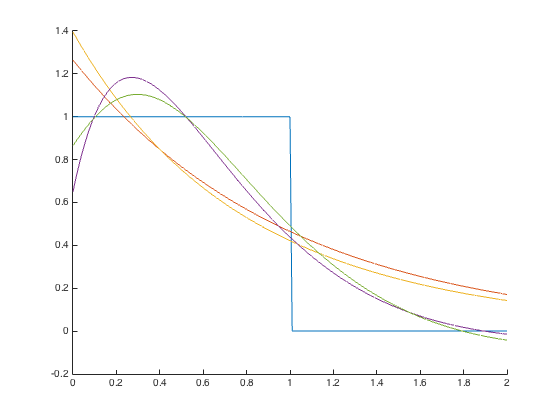
\includegraphics[scale=.3]{Figures/01_6.png}
                \lstinputlisting[Language=Matlab, firstline=11]{H01.m}
        \end{enumerate}
\end{enumerate}
\end{document}
